% chap4.tex (Customer Description)

\chapter{Customer Description} 

In this chapter, I will describe the customers present in the PowerTAC simulation system and some statistics their attributes.

\section{Customer Categories}


In Power TAC simulation, a customer can be electricity consumer or producer based on the power type it has. A customer evaluates the tariff plans targetted for its power type and can look for the tariff that gives it maximum monetary benefit. There are several types of customers in the Power TAC simulation such as consumption, interruptible consumption, thermal storage, solar production, wind production and electric vehicle. Each power type has its own characterstics. For example, interruptile consumption customers can shift their electricity demand to some off peak hour, the solar production customers can produce energy based on the weather condition. As opposed to previous methods on demand forecasting, I argue that each category of customers based on the power type should be treated differently. One load forecasting method can be suitable for a category of customers while it may be unsuitable for other categories because each category behaves differently. In the below section, I describe the characterstics of the customers.

\begin{itemize}
\item \textbf{Consumption: } A customer with power type consumption are the most common customers. They use the energy when they need it. They cannot shift their demand to a future timeslot. Usually, they have a regular pattern of their energy usage. Often, they show a similar pattern for weekdays. They have similar kind of usage pattern for the weekends. 



\item \textbf{Interruptible Consumption: }
Interruptible customers are smart enough to shift their energy demand in a timeslot where they can buy electricity at a reduced price. Because of this shifting capability, they don't show a regular usage pattern as the consumption customers do. 

\item \textbf{Thermal Storage: }
Thermal storage customers show a weekly pattern in their electricity usage. Also, during a day, their electricity usage in a day depends  much on the energy they used in the last timeslot. 


\item \textbf{Solar Production}
The solar energy production customer's energy production depends on the cloud cover. They are highly likely to produce energy during the day time.

\item\textbf{Wind Production} Wind production customers generate energy from the wind.
\item \textbf{Electric Vehicle} An electric vehicle customer represents one electric vehicle. Their usage of energy is quite irregular and hard to predict. \\
\end{itemize}

 To discuss the behavior of different power typed ustomers, a representative customer was chosen from each type. The table \ref{table:repCust} shows the customer chosen to discuss -

\begin{table}[h!]
\centering
\begin{tabular}{ |c|c| } 
\hline
Power Type & Customer Name \\
\hline
Consumption & downtown offices \\ 
Interruptible Consumption & village 1 ns \\ 
Thermal Storage & sf2 \\ 
Solar Production & sunnyHill \\ 
Wind Production & windmill 1 \\ 
Electric Vehicle & high income 1 \\ 
\hline
\end{tabular}
\caption{Representative customer from each power type}
\label{table:repCust}
\end{table}

Before diving into the problem of solving forecasting methods, I found it useful to take a look at how the customers behave. The log extractor program extracts all the energy consumption and production by all the customer on all the timeslot. At the end of the game, it makes a report on normalized usage of all the customers in all the week slots. Normalized values are useful because even if the amount of energy usage vary, the pattern of usage can be captured through it. The figures \ref{fig:daily1} to \ref{fig:daily3}, shows normalized electricity demand or supply of Mondays. 0 in the x axis means hour 12:00 am. From the figures \ref{fig:daily1} to \ref{fig:daily3}, it is clear that some customer's electricity usage is higly correlated with time of the hour of the day. The customers of type consumption and solar energy can be example of these types. The other customer types demands did not seem to have correlation with hour of a day. In both consumption and solar energy customers the consumption or production curve grew smoothly till it reached a peak point. After the reaching the peak, the production or consumption reduced smoothly. It is clear that the customers with types interruptible consumption, wind production, thermal storage and electric vehicle had irregular demand/supply pattern. 

In figure \ref{fig:weekly1} to \ref{fig:weekly3}, normalized usage during the week is shown. Hour 0 to 23 represents all the hours of Monday from 12:00 am to 11:00 pm. It appears that, the electricity demand for consumption customer, interruptible consumption, thermal storage had repeatative demand pattern everyday. The  solar energy production customer showed repeatative production pattern. Moreover some customers such as the consumption type and the thermal storage type showed different pattern during the weekend. During the weekend they usually had lower energy demand than the weekdays. In the case of electric vehicle and wind energy production customers the demand/supply patterns were not regular. From these observation, it can be assumed that the consumption customer and the solar energy type customers can be forecasted with the most accuracy. Due to irregular patterns of other customers, they will be harder to make forecast about accurately.
 
% figure start
\begin{figure}[!h]
\centering
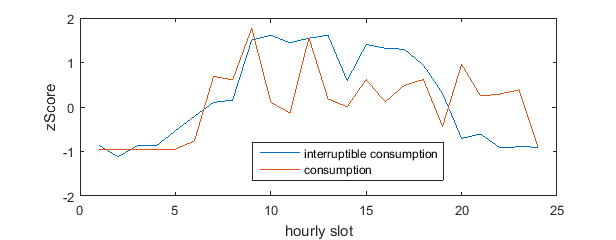
\includegraphics{daily1.png}
\caption{Caption 1}
\label{fig:daily1}
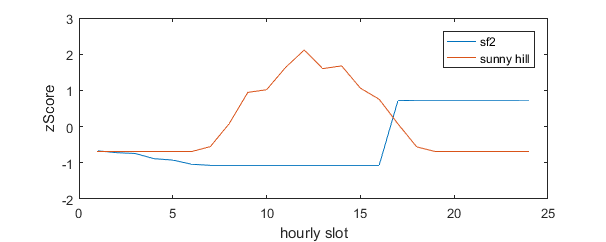
\includegraphics{daily2.png}
\caption{Caption 1}
\label{fig:daily2}
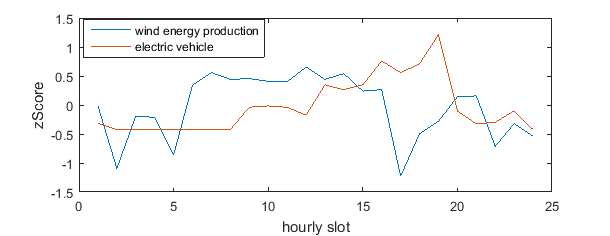
\includegraphics{daily3.png}
\caption{Caption 1}
\label{fig:daily3}
\end{figure}

\begin{figure}[!h]
\centering
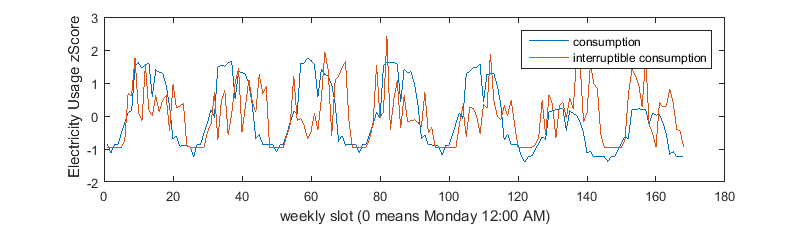
\includegraphics{weekly1.png}
\caption{Caption 1}
\label{fig:weekly1}
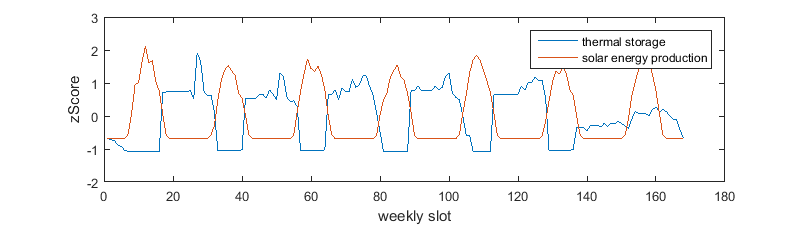
\includegraphics{weekly2.png}
\caption{Caption 1}
\label{fig:weekly2}
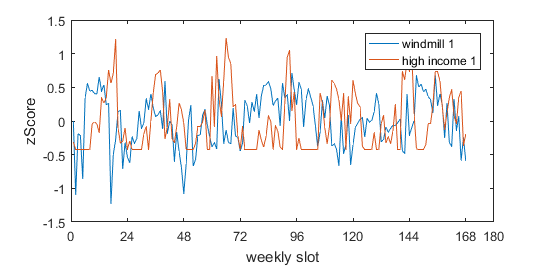
\includegraphics{weekly3.png}
\caption{Caption 1}
\label{fig:weekly3}
\end{figure}

%figure end

\section{Statistics}
In this section, I present some statistics on the customers available in the system. 

\begin{itemize}
\item \textbf{Customer Vs PowerType}

In the figure \ref{fig:cust-pt} we can see the system has more customer with the power type electric vehicle than any other power types. This is because the electric vehicle represents a population of size 1.

\item \textbf{Population Vs PowerType}
From figure \ref{fig:pop-pt} by far the powertype of consumption has the most number of population.

\item \textbf{Total Energy Consumed Vs PowerType}
From figure \ref{fig:energy-pt} we can see that the consumption type customers uses the most amount of the electricity.


\begin{figure}
\centering
\begin{minipage}{.5\textwidth}
  \centering
  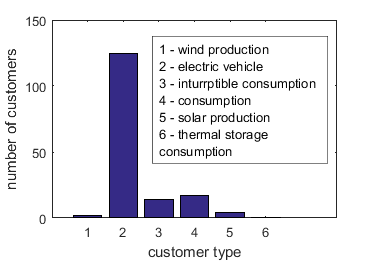
\includegraphics[width=\linewidth]{4-customer-vs-powertype.jpg}
  \caption{Number of customers vs Powertype.}
  \label{fig:cust-pt}
\end{minipage}%
\begin{minipage}{.5\textwidth}
  \centering
  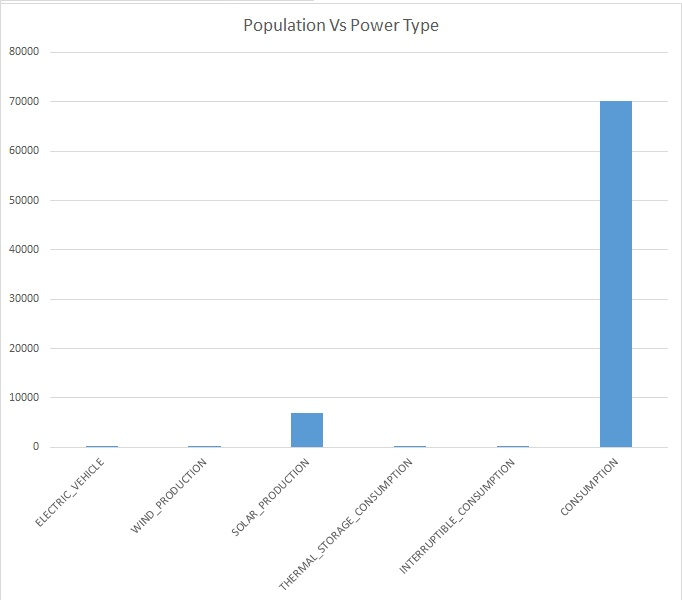
\includegraphics[width=\linewidth]{2-population-vs-powertype.jpg}
  \caption{Population vs Powertype}
  \label{fig:pop-pt}
\end{minipage}

\centering
\begin{minipage}{.5\textwidth}
  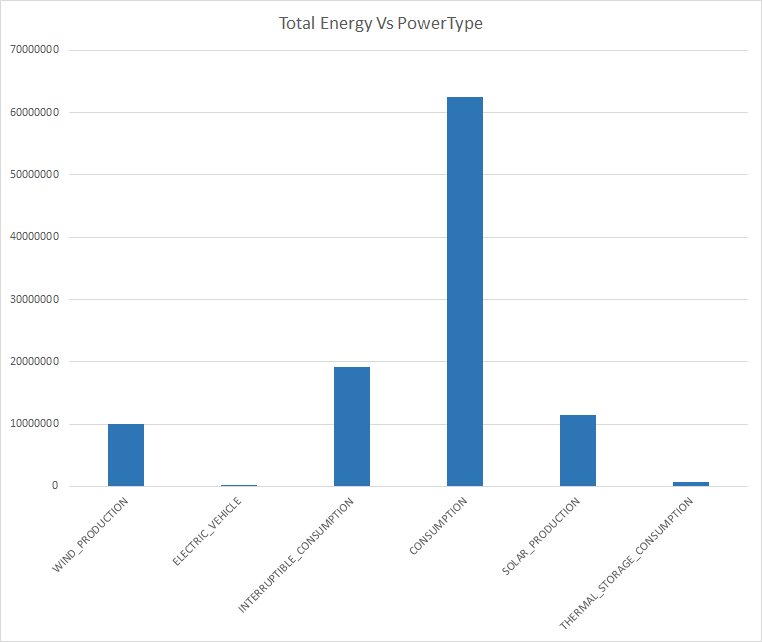
\includegraphics[width=\linewidth]{3-energy-vs-powertype.png}
  \caption{Energy vs PowerType.}
  \label{fig:energy-pt}
\end{minipage}%
\begin{minipage}{.5\textwidth}
  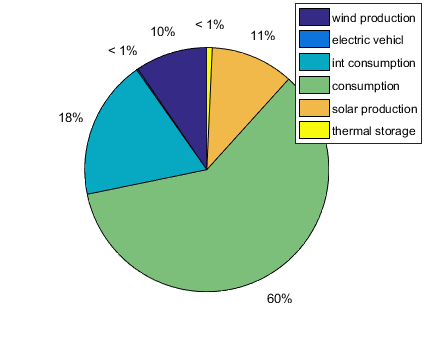
\includegraphics[width=\linewidth]{pie-energy-share.png}
  \caption{Energy share for each power type.}
  \label{fig:energy-shares}
\end{minipage}

\end{figure}

\end{itemize}
